%~~~~~~~~~~~~~~~~~~~~~~~~~~~~~~~~~~~~~~~~~~~~~~~~~~~~~~~~~~~~~~~~~~~~~
%    File      : rt_cap1
%~~~~~~~~~~~~~~~~~~~~~~~~~~~~~~~~~~~~~~~~~~~~~~~~~~~~~~~~~~~~~~~~~~~~~

Primeiro capítulo do relatório\index{relatório técnico}. A partir desse ponto, você é livre para incluir seções, subseções e subsubseções.

Você pode incluir citações on line\index{citação!on line}, como \citeonline{macedo_information_2014}. Ou não \cite{lima-marques_outline_2011}.

A \autoref{tab:teste} -- \nameref{tab:teste} é somente um exemplo.\index{tabela}

\begin{longtable}{c | p{10cm} | r }
    % Título da tabela
    \caption[Teste]{Teste de uma tabela}\label{tab:teste} \\

    % -------------------------------------------------
    % Cabeçalho
    \toprule
    \textbf{Item} & \multicolumn{1}{c|}{\textbf{Descrição}} & \multicolumn{1}{c}{\textbf{Valor}} \\ \midrule \endfirsthead

    \toprule
    \textbf{Item} & \multicolumn{1}{c|}{\textbf{Descrição}} & \multicolumn{1}{c}{\textbf{Valor}} \\ \midrule \endhead
    % -------------------------------------------------

    % -------------------------------------------------
    % Corpo
    1 & Item qualquer para testar inclusive a quebra de parágrafos, por isso esse texto é tão grande e chato &
    R\$ 1.000.000,00 \\ \hline
    
    2 & Outro texto, agora pequeno &
    R\$ 2.000.000,00 \\ \hline
    
    3 & Mais um texto pequeno &
    R\$ 500.000,00 \\ \hline
    
    \multicolumn{2}{r|}{\emph{Total:}} & R\$ 3.500.000,00 \\ \bottomrule
    
    % -------------------------------------------------
    % Citação da fonte
    \multicolumn{3}{l}{\footnotesize Fonte: Equipe de pesquisa -- CPAI} \\

\end{longtable}

E que tal uma figura? A \autoref{fig:maia} -- \nameref{fig:maia} faz isso! 

\begin{figure}[h!]
    \centering
    \caption[MAIA]{\MAIA\ -- \maia} \label{fig:maia}
    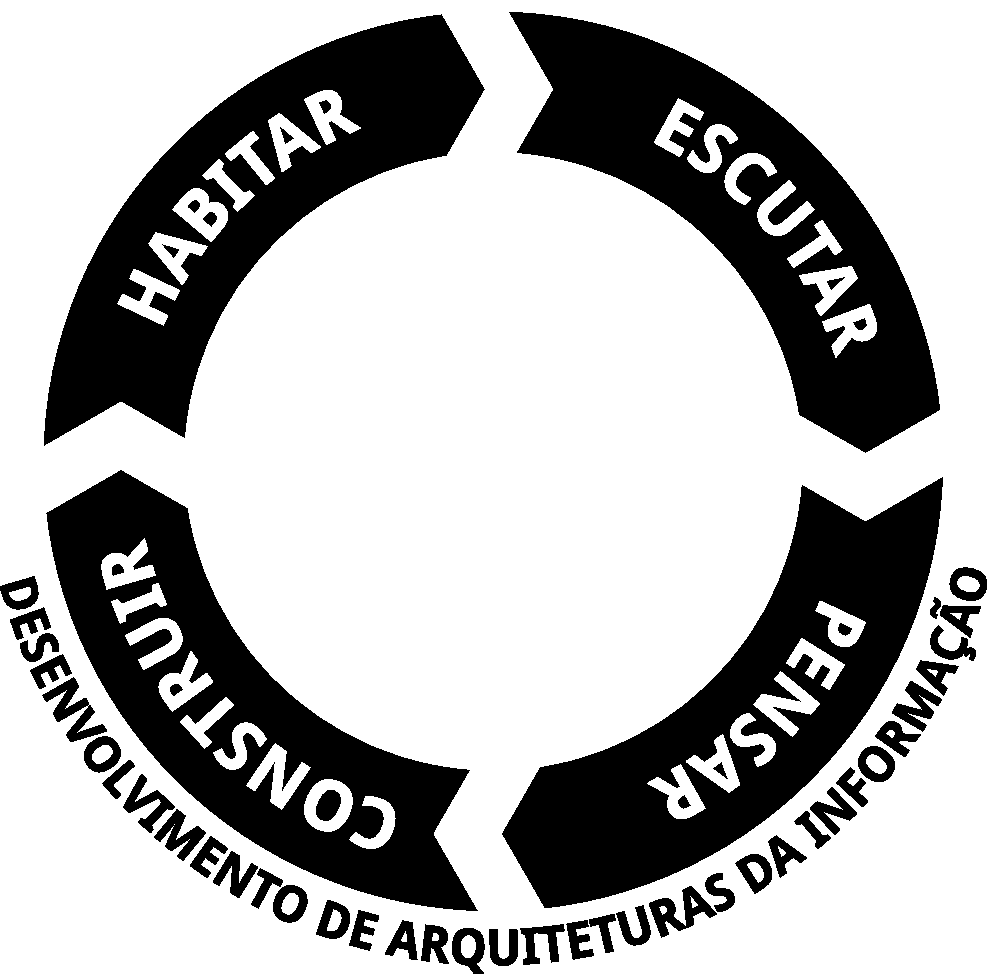
\includegraphics[width=0.4\linewidth,frame=0.5pt 5pt]{img/maia}
    \fonte{Equipe de pesquisa -- CPAI}
\end{figure}

% Texto genérico para visualizar quebra de páginas, cabeçalhos, rodapés e outros itens de formatação
\lipsum[2-3]

\lipsum[5-8]
